% Template for PLoS
% Version 3.2 March 2016
%
% % % % % % % % % % % % % % % % % % % % % %
%
% -- IMPORTANT NOTE
%
% This template contains comments intended 
% to minimize problems and delays during our production 
% process. Please follow the template instructions
% whenever possible.
%
% % % % % % % % % % % % % % % % % % % % % % % 
%
% Once your paper is accepted for publication, 
% PLEASE REMOVE ALL TRACKED CHANGES in this file 
% and leave only the final text of your manuscript. 
% PLOS recommends the use of latexdiff to track changes during review, as this will help to maintain a clean tex file.
% Visit https://www.ctan.org/pkg/latexdiff?lang=en for info or contact us at latex@plos.org.
%
%
% There are no restrictions on package use within the LaTeX files except that 
% no packages listed in the template may be deleted.
%
% Please do not include colors or graphics in the text.
%
% The manuscript LaTeX source should be contained within a single file (do not use \input, \externaldocument, or similar commands).
%
% % % % % % % % % % % % % % % % % % % % % % %
%
% -- FIGURES AND TABLES
%
% Please include tables/figure captions directly after the paragraph where they are first cited in the text.
%
% DO NOT INCLUDE GRAPHICS IN YOUR MANUSCRIPT
% - Figures should be uploaded separately from your manuscript file. 
% - Figures generated using LaTeX should be extracted and removed from the PDF before submission. 
% - Figures containing multiple panels/subfigures must be combined into one image file before submission.
% For figure citations, please use "Fig" instead of "Figure".
% See http://journals.plos.org/plosone/s/figures for PLOS figure guidelines.
%
% Tables should be cell-based and may not contain:
% - tabs/spacing/line breaks within cells to alter layout or alignment
% - vertically-merged cells (no tabular environments within tabular environments, do not use \multirow)
% - colors, shading, or graphic objects
% See http://journals.plos.org/plosone/s/tables for table guidelines.
%
% For tables that exceed the width of the text column, use the adjustwidth environment as illustrated in the example table in text below.
%
% % % % % % % % % % % % % % % % % % % % % % % %
%
% -- EQUATIONS, MATH SYMBOLS, SUBSCRIPTS, AND SUPERSCRIPTS
%
% IMPORTANT
% Below are a few tips to help format your equations and other special characters according to our specifications. For more tips to help reduce the possibility of formatting errors during conversion, please see our LaTeX guidelines at http://journals.plos.org/plosone/s/latex
%
% For inline equations, please be sure to include all portions of an equation in the math environment.  For example, x$^2$ is incorrect; this should be formatted as $x^2$ (or $\mathrm{x}^2$ if the romanized font is desired).
%
% Do not include text that is not math in the math environment. For example, CO2 should be written as CO\textsubscript{2} instead of CO$_2$.
%
% Please add line breaks to long display equations when possible in order to fit size of the column. 
%
% For inline equations, please do not include punctuation (commas, etc) within the math environment unless this is part of the equation.
%
% When adding superscript or subscripts outside of brackets/braces, please group using {}.  For example, change "[U(D,E,\gamma)]^2" to "{[U(D,E,\gamma)]}^2". 
%
% Do not use \cal for caligraphic font.  Instead, use \mathcal{}
%
% % % % % % % % % % % % % % % % % % % % % % % % 
%
% Please contact latex@plos.org with any questions.
%
% % % % % % % % % % % % % % % % % % % % % % % %

\documentclass[10pt,letterpaper]{article}
\usepackage[top=0.85in,left=2.75in,footskip=0.75in]{geometry}


%% %%%%%%%%%%%%%%%%%%%%%%%%%%%%%%%%%%%%%%%%%%%%%%%%%%%%%%%%%%%%%%%%%%%%%%%%%%
%%                        Template paackages
%% %%%%%%%%%%%%%%%%%%%%%%%%%%%%%%%%%%%%%%%%%%%%%%%%%%%%%%%%%%%%%%%%%%%%%%%%%%
% Use adjustwidth environment to exceed column width (see example table in text)
\usepackage{changepage}

% Use Unicode characters when possible
\usepackage[utf8x]{inputenc}

% textcomp package and marvosym package for additional characters
\usepackage{textcomp,marvosym}

% fixltx2e package for \textsubscript
\usepackage{fixltx2e}

% amsmath and amssymb packages, useful for mathematical formulas and symbols
\usepackage{amsmath,amssymb}

% cite package, to clean up citations in the main text. Do not remove.
\usepackage{cite}

% Use nameref to cite supporting information files (see Supporting Information section for more info)
\usepackage{nameref,hyperref}

% line numbers
\usepackage[right]{lineno}

% ligatures disabled
\usepackage{microtype}
\DisableLigatures[f]{encoding = *, family = * }

% Remove comment for double spacing
%\usepackage{setspace} 
%\doublespacing

% Text layout
\raggedright
\setlength{\parindent}{0.5cm}
\textwidth 5.25in 
\textheight 8.75in

% Bold the 'Figure #' in the caption and separate it from the title/caption with a period
% Captions will be left justified
\usepackage[aboveskip=1pt,labelfont=bf,labelsep=period,justification=raggedright,singlelinecheck=off]{caption}
\renewcommand{\figurename}{Fig}

% Use the PLoS provided BiBTeX style
\bibliographystyle{plos2015}

% Remove brackets from numbering in List of References
\makeatletter
\renewcommand{\@biblabel}[1]{\quad#1.}
\makeatother

% Leave date blank
\date{}

% Header and Footer with logo
\usepackage{lastpage,fancyhdr,graphicx}
\usepackage{epstopdf}
\pagestyle{myheadings}
\pagestyle{fancy}
\fancyhf{}
\setlength{\headheight}{27.023pt}
\lhead{
\includegraphics[width=2.0in]{PLOS-submission.eps}}
\rfoot{\thepage/\pageref{LastPage}}
\renewcommand{\footrule}{\hrule height 2pt \vspace{2mm}}
\fancyheadoffset[L]{2.25in}
\fancyfootoffset[L]{2.25in}
\lfoot{\sf PLOS}

%% Include all macros below

\newcommand{\lorem}{{\bf LOREM}}
\newcommand{\ipsum}{{\bf IPSUM}}

%% %%%%%%%%%%%%%%%%%%%%%%%%%%%%%%%%%%%%%%%%%%%%%%%%%%%%%%%%%%%%%%%%%%%%%%%%%%
%%                         CUSTOM PACKAGES
%% %%%%%%%%%%%%%%%%%%%%%%%%%%%%%%%%%%%%%%%%%%%%%%%%%%%%%%%%%%%%%%%%%%%%%%%%%%
\usepackage{color}
\usepackage{subfig}
%% END MACROS SECTION

\newcommand{\todo}[1]{[{\color{red}\textit{todo}\textit{: #1}}]}
 
\begin{document}
\vspace*{0.2in}

% Title must be 250 characters or less.
\begin{flushleft}
{\Large
\textbf\newline{How Not to Forecast the Flu} % Please use "title case" (capitalize all terms in the title except conjunctions, prepositions, and articles).
}
\newline
% Insert author names, affiliations and corresponding author email (do not include titles, positions, or degrees).
\\
Prithwish Chakraborty\textsuperscript{1,2*},
Bryan Lewis\textsuperscript{3},
Stephen Eubank\textsuperscript{3},
John S. Brownstein\textsuperscript{4,5},
Madhav Marathe\textsuperscript{2,3}, and
Naren Ramakrishnan\textsuperscript{1,2},
\\
\bigskip
\textbf{1} Discovery Analytics Center, Virginia Tech, VA, USA\\
\textbf{2} Dept.\ of Computer Science, Virginia Tech, VA, USA\\
\textbf{3} Network Dynamics and Simulation Science Laboratory, Biocomplexity Institute, Virginia Tech, VA, USA\\
\textbf{4} Children's Hospital Informatics Program, Boston Children’s Hospital, MA, USA\\
\textbf{5} Dept.\ of Pediatrics, Harvard Medical School, MA, USA\\
\bigskip

% Insert additional author notes using the symbols described below. Insert symbol callouts after author names as necessary.
% 
% Remove or comment out the author notes below if they aren't used.
%
% Primary Equal Contribution Note
% \Yinyang These authors contributed equally to this work.

% Additional Equal Contribution Note
% Also use this double-dagger symbol for special authorship notes, such as senior authorship.
% \ddag These authors also contributed equally to this work.

% Current address notes
% \textcurrency Current Address: Dept/Program/Center, Institution Name, City, State, Country % change symbol to "\textcurrency a" if more than one current address note
% \textcurrency b Insert second current address 
% \textcurrency c Insert third current address

% Deceased author note
% \dag Deceased

% Group/Consortium Author Note
% \textpilcrow Membership list can be found in the Acknowledgments section.

% Use the asterisk to denote corresponding authorship and provide email address in note below.
* prithwi@vt.edu

\end{flushleft}
% Please keep the abstract below 300 words
\section*{Summary}
Accurate and timely influenza (flu) forecasting has gained significant traction
in recent times. If done well, such forecasting can aid in deploying effective
public health measures. Unlike other statistical or machine learning problems,
however, flu forecasting brings unique challenges and considerations stemming
from the nature of the surveillance apparatus and the end-utility of forecasts.
This article presents a set of considerations for flu modelers that must be
addressed for effective and useful forecasting.


% Please keep the Author Summary between 150 and 200 words
% Use first person. PLOS ONE authors please skip this step. 
% Author Summary not valid for PLOS ONE submissions.   
% \section*{Author Summary}

\linenumbers

% Use "Eq" instead of "Equation" for equation citations.
\section*{Introduction}
As the current flu season dwindles and we prepare to embark upon a new flu
season in a few months, we will hear the usual cautionary notes about
vaccinations, the preparedness of our health systems, and the specific strains
that are relevant for these seasons.  Recent competitions, organized by
agencies like the CDC and IARPA, have spurred interest in flu forecasting
across academia and industry. While the CDC competition aimed to forecast flu
seasonal characteristics in the US, the IARPA Open Source Indicators (OSI)
forecasting tournament was focused on disease forecasting (flu and rare
diseases) in countries of Latin America. Our team was declared the winner in
the IARPA OSI competition and our goal here is to communicate our lessons
learned about what goes into a successful forecasting engine while ensuring its
relevance to public health policy and, consider some common assumptions that
can be violated and require careful attention. Broadly, such considerations 
can be categorized with respect to  `Surveillance Characteristics' 
(see Fig~\ref{fig1})
and `Forecasting Practices' (see Fig~\ref{fig2}), as discussed below.

% Place figure captions after the first paragraph in which they are cited.
% \begin{figure}[!h]
% \caption{{\bf Bold the figure title.}
% Figure Caption Proin rutrum vel massa non gravida. Quisque tempor sem et dignissim rutrum. A: Lorem ipsum dolor sit amet. B: Consectetur adipiscing elit.}
% \label{fig1}
% \end{figure}

% Results and Discussion can be combined.
\begin{figure}[!h]
  % \centering
  % \subfloat[Between surveillance difference\label{1a}]{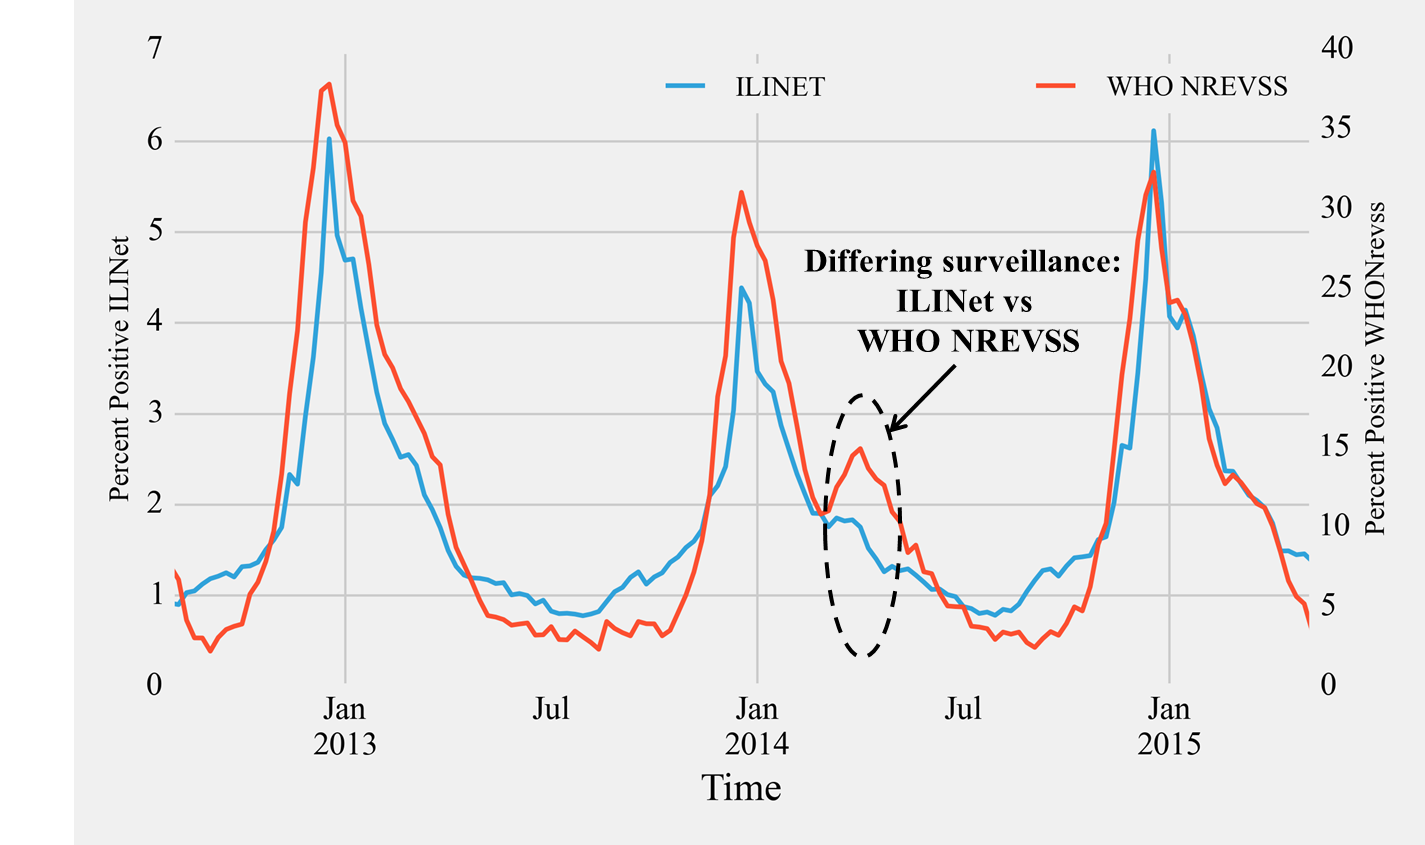
\includegraphics[width=0.45\textwidth]{./figs/ilinet_vs_who.png}} 
    % \hspace{0.5em}
  % \subfloat[Between strains difference\label{1b}]{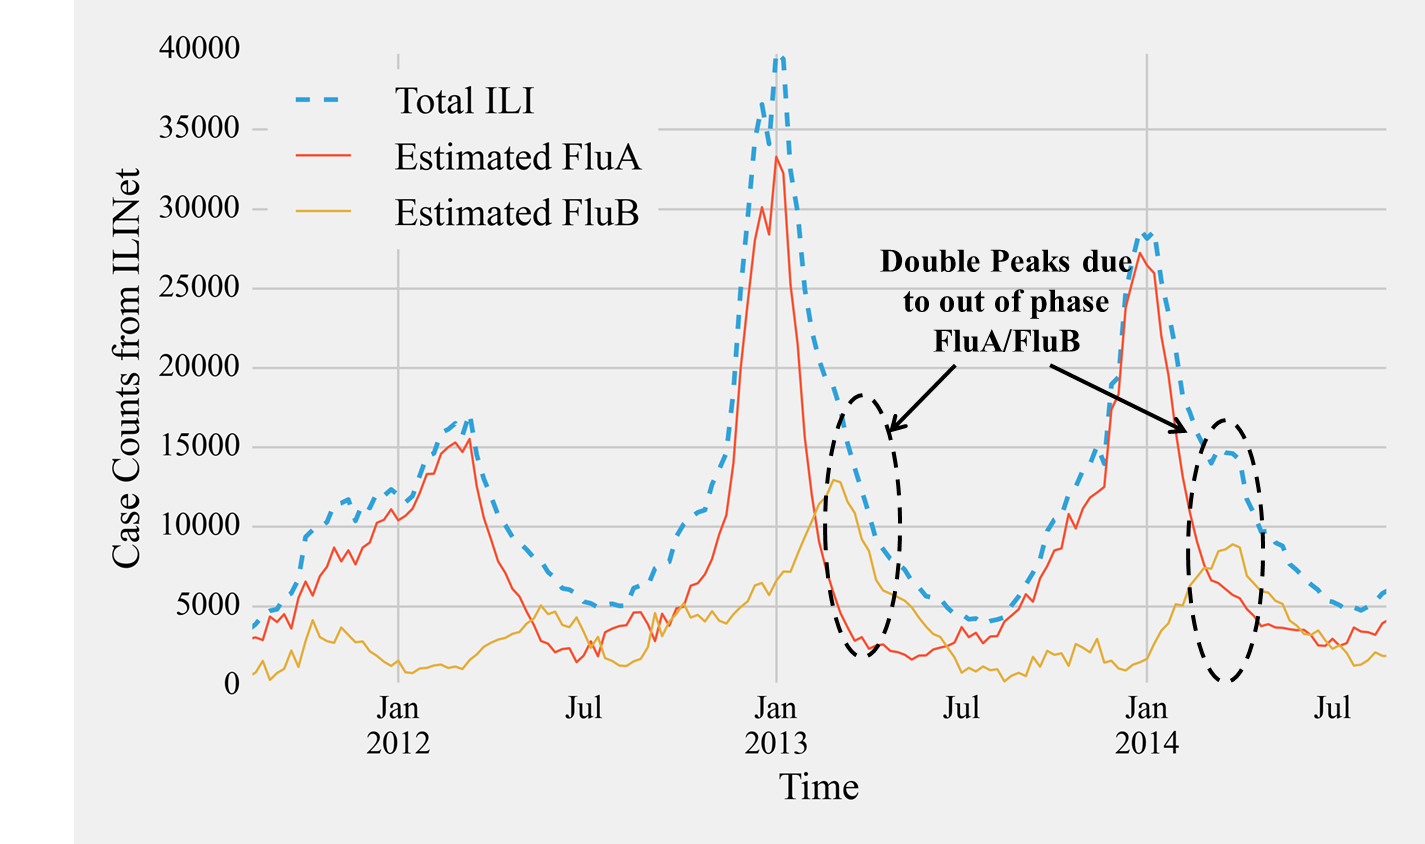
\includegraphics[width=0.45\textwidth]{./figs/ilinet_subtyped.png}} 
    % \\
  % \subfloat[Surveillance Instability\label{1c}]{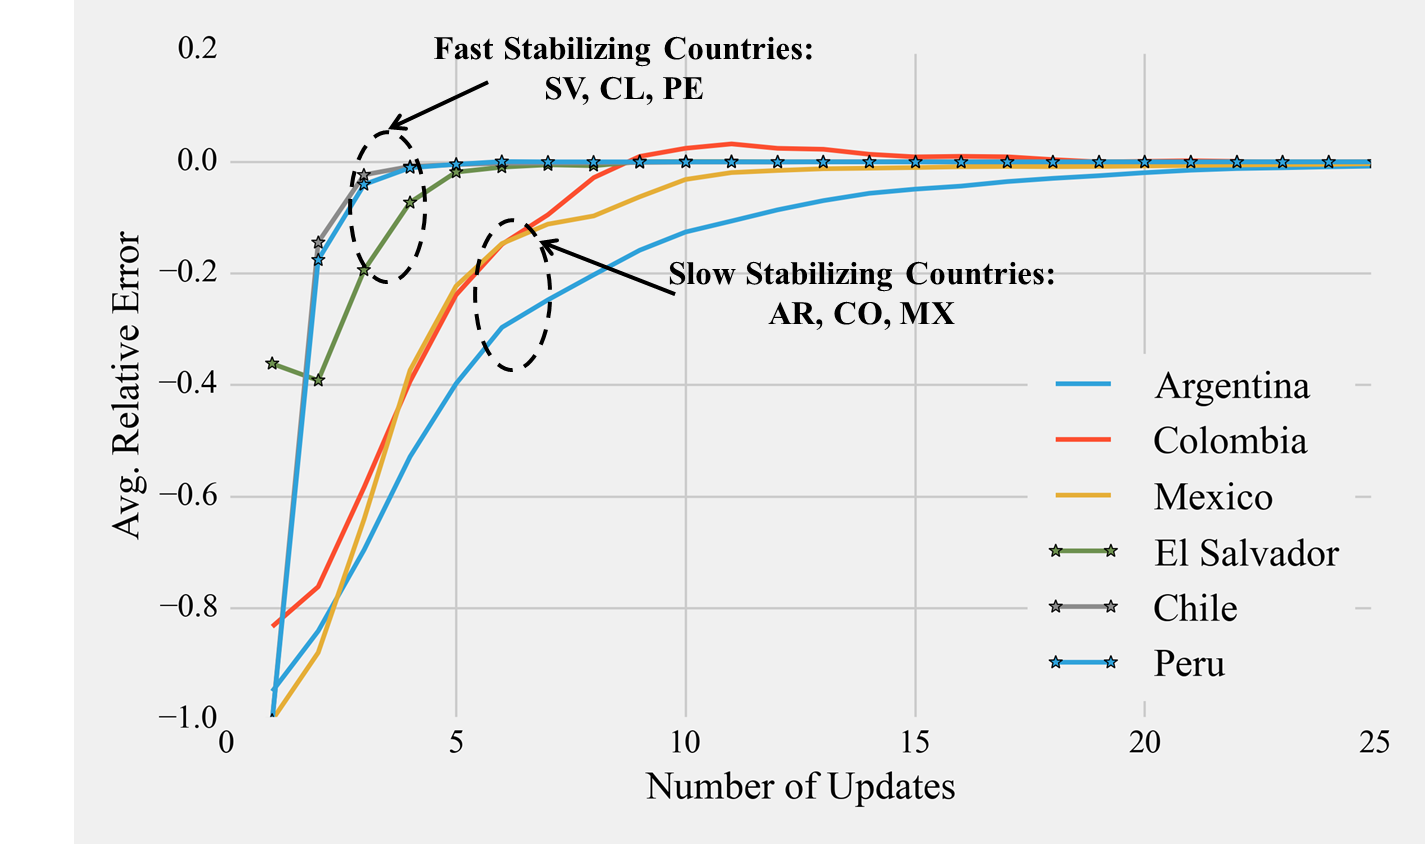
\includegraphics[width=0.45\textwidth]{./figs/ilinet_update.png}}
    % \hspace{0.5em}
  % \subfloat[Surveillance drop-off\label{1d}]{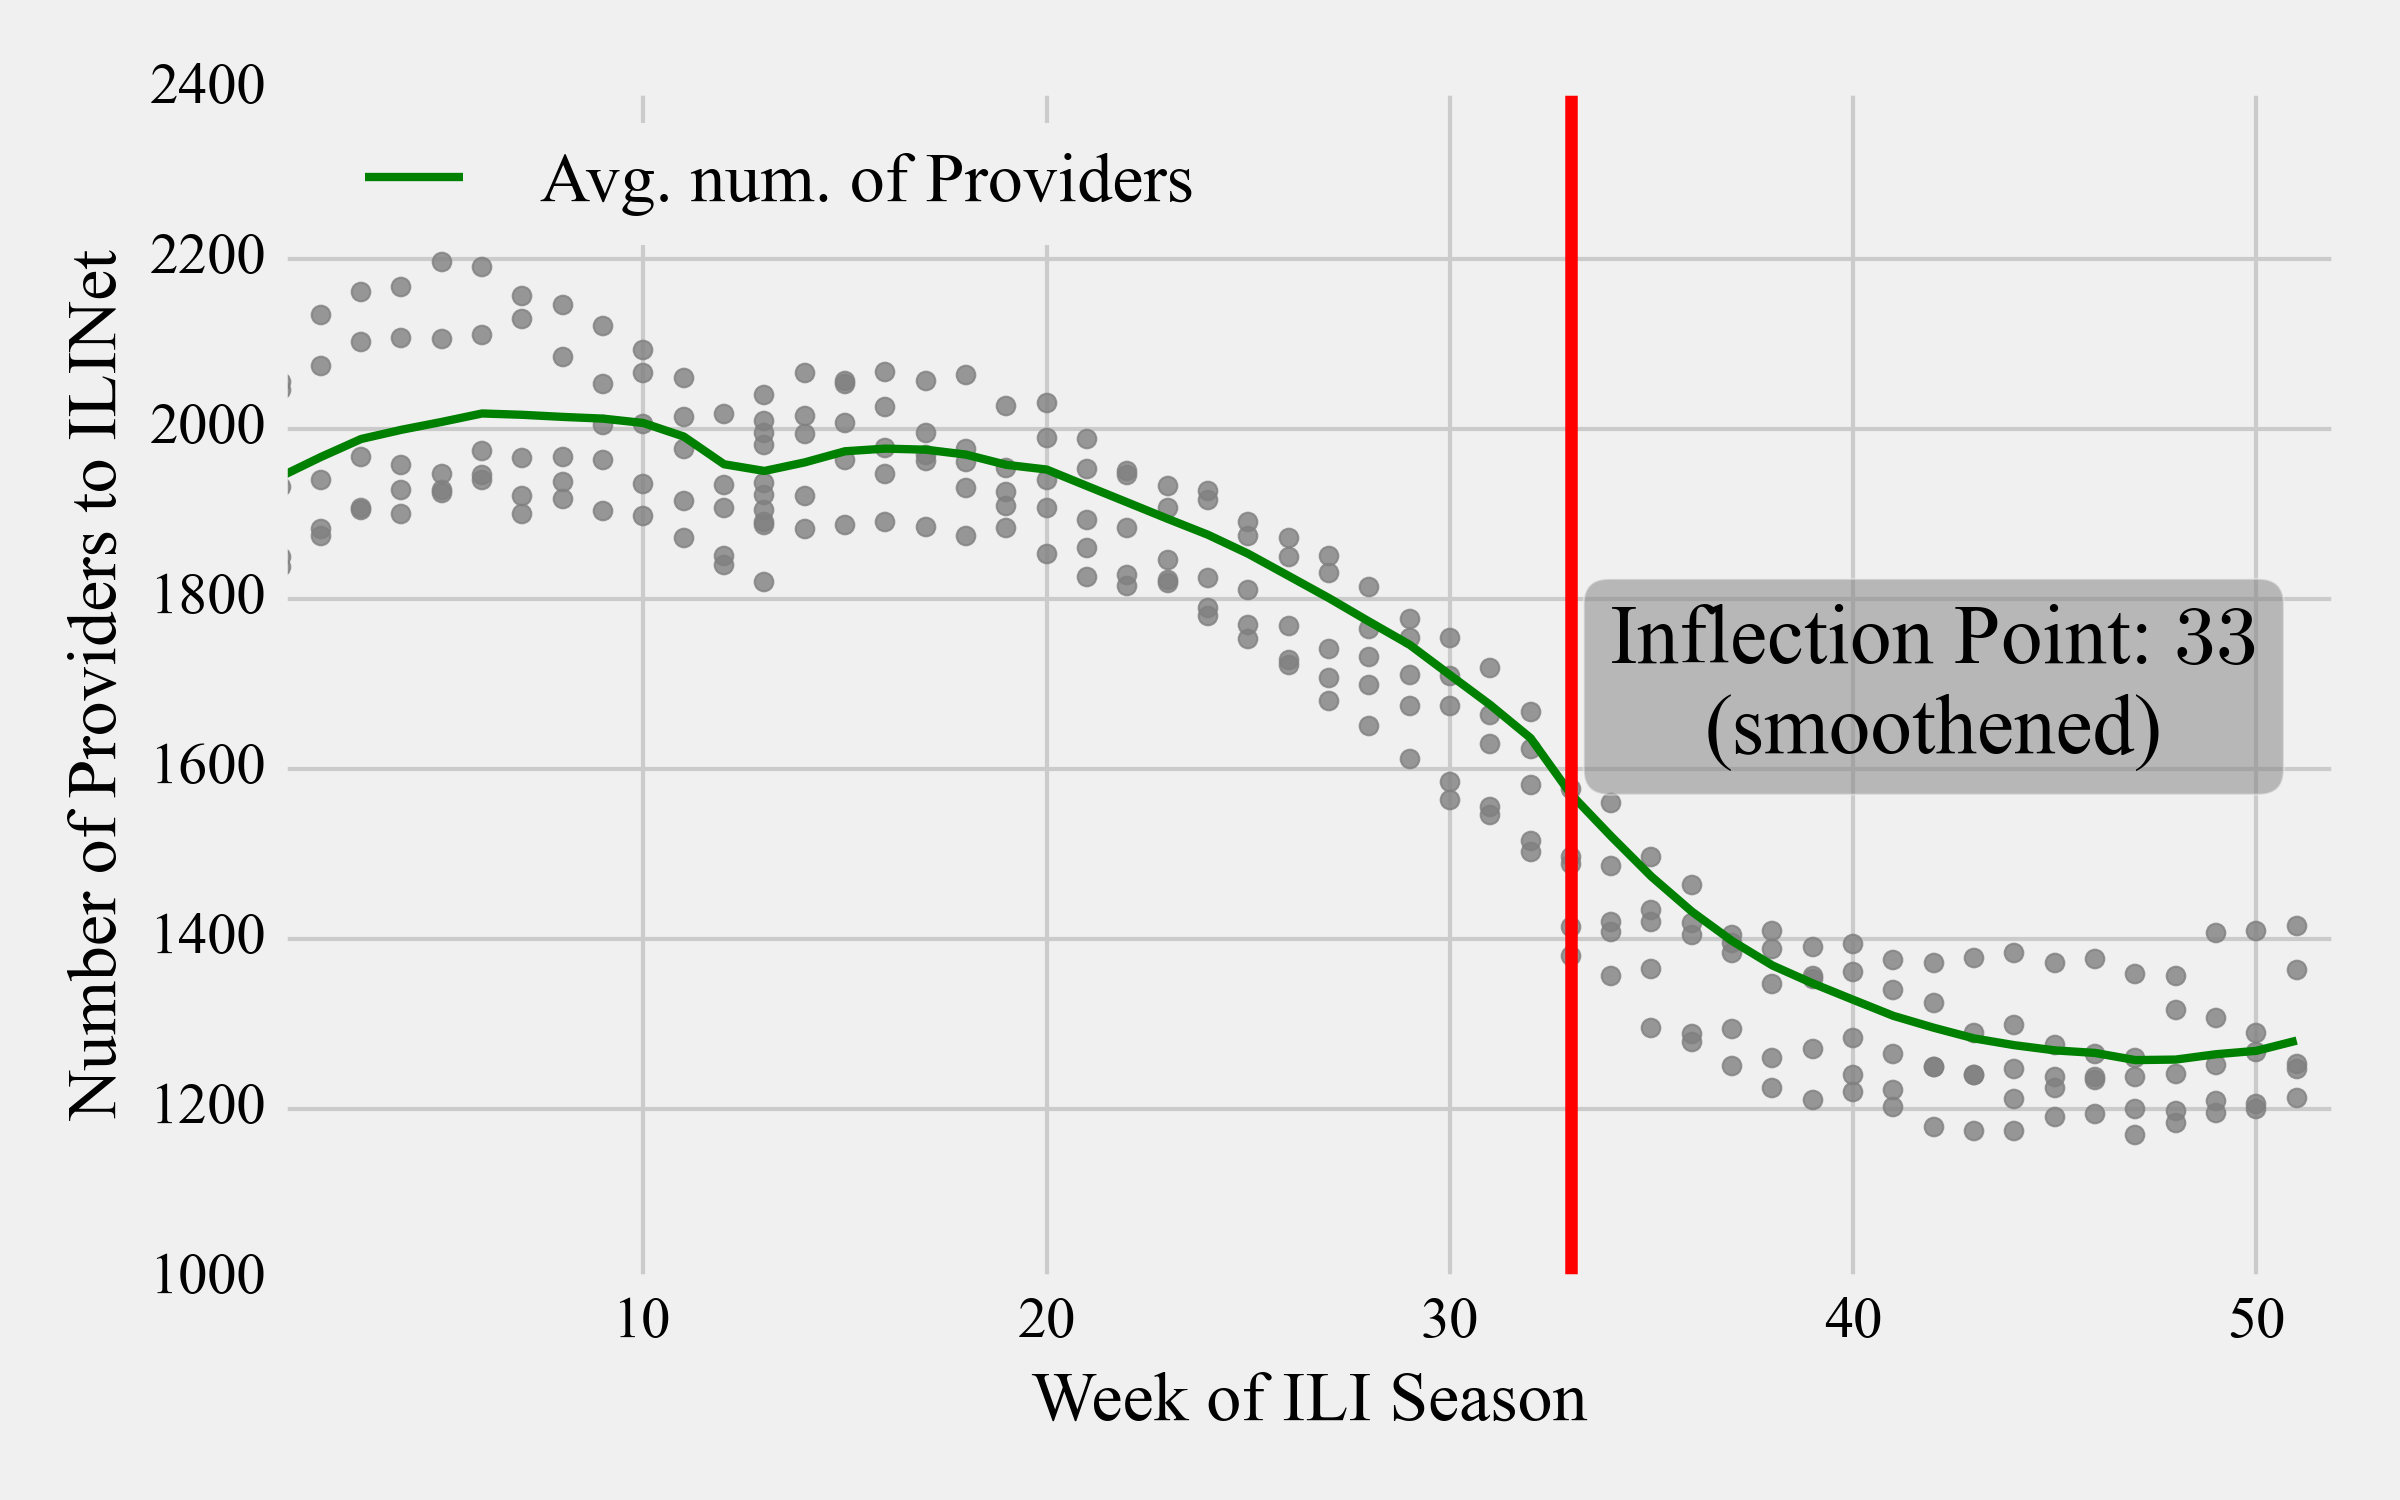
\includegraphics[width=0.45\textwidth]{./figs/ili_surveillance_drop.png}} 
  \centering
  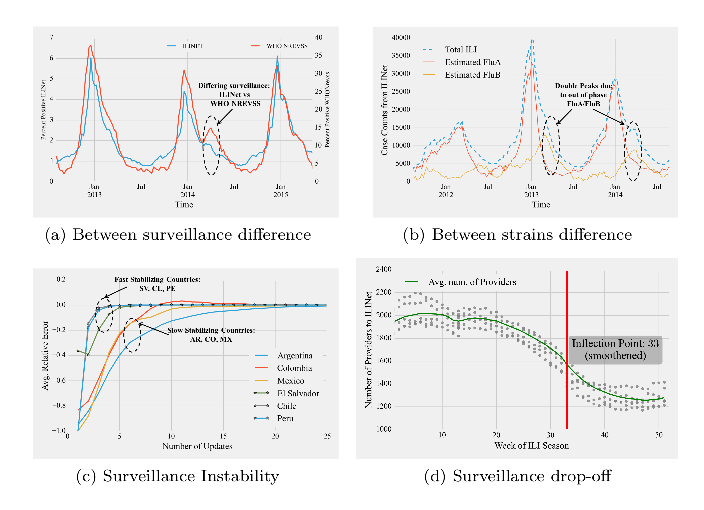
\includegraphics[width=0.96\linewidth]{./figs/char_figs.eps}

  \caption{\textbf{Different Characteristics of Surveillance systems.}
  (a)  Phase differences in reported ILI percentages between two 
  surveillance systems(ILINet vs WHO NREVSS).
  (b)  Phase differences between different ILI substrains 
  (Flu A vs Flu B) leading to double peaked overall ILI curve.
  (c) Surveillance reports unstable many weeks after first report.
  While countries like Chile stabilizes quickly (within 5 weeks), 
  other countries like Argentina stabilizes after many weeks ($\geq 10$). 
  (d) Surveillance drop-off towards the end of the season - scatter plot of 
  Number of providers reporting to CDC ILINet as a function of ILI season 
  week. Green Line shows the smoothened average while the red vertical
  line shows the smoothened inflection point of surveillance coverage. 
  (Smoothing interval = 4)
  \label{fig1}
  }
\end{figure}

\begin{figure}[t]
  \centering
  % \subfloat[Single source prediction accuracy\label{2a}]{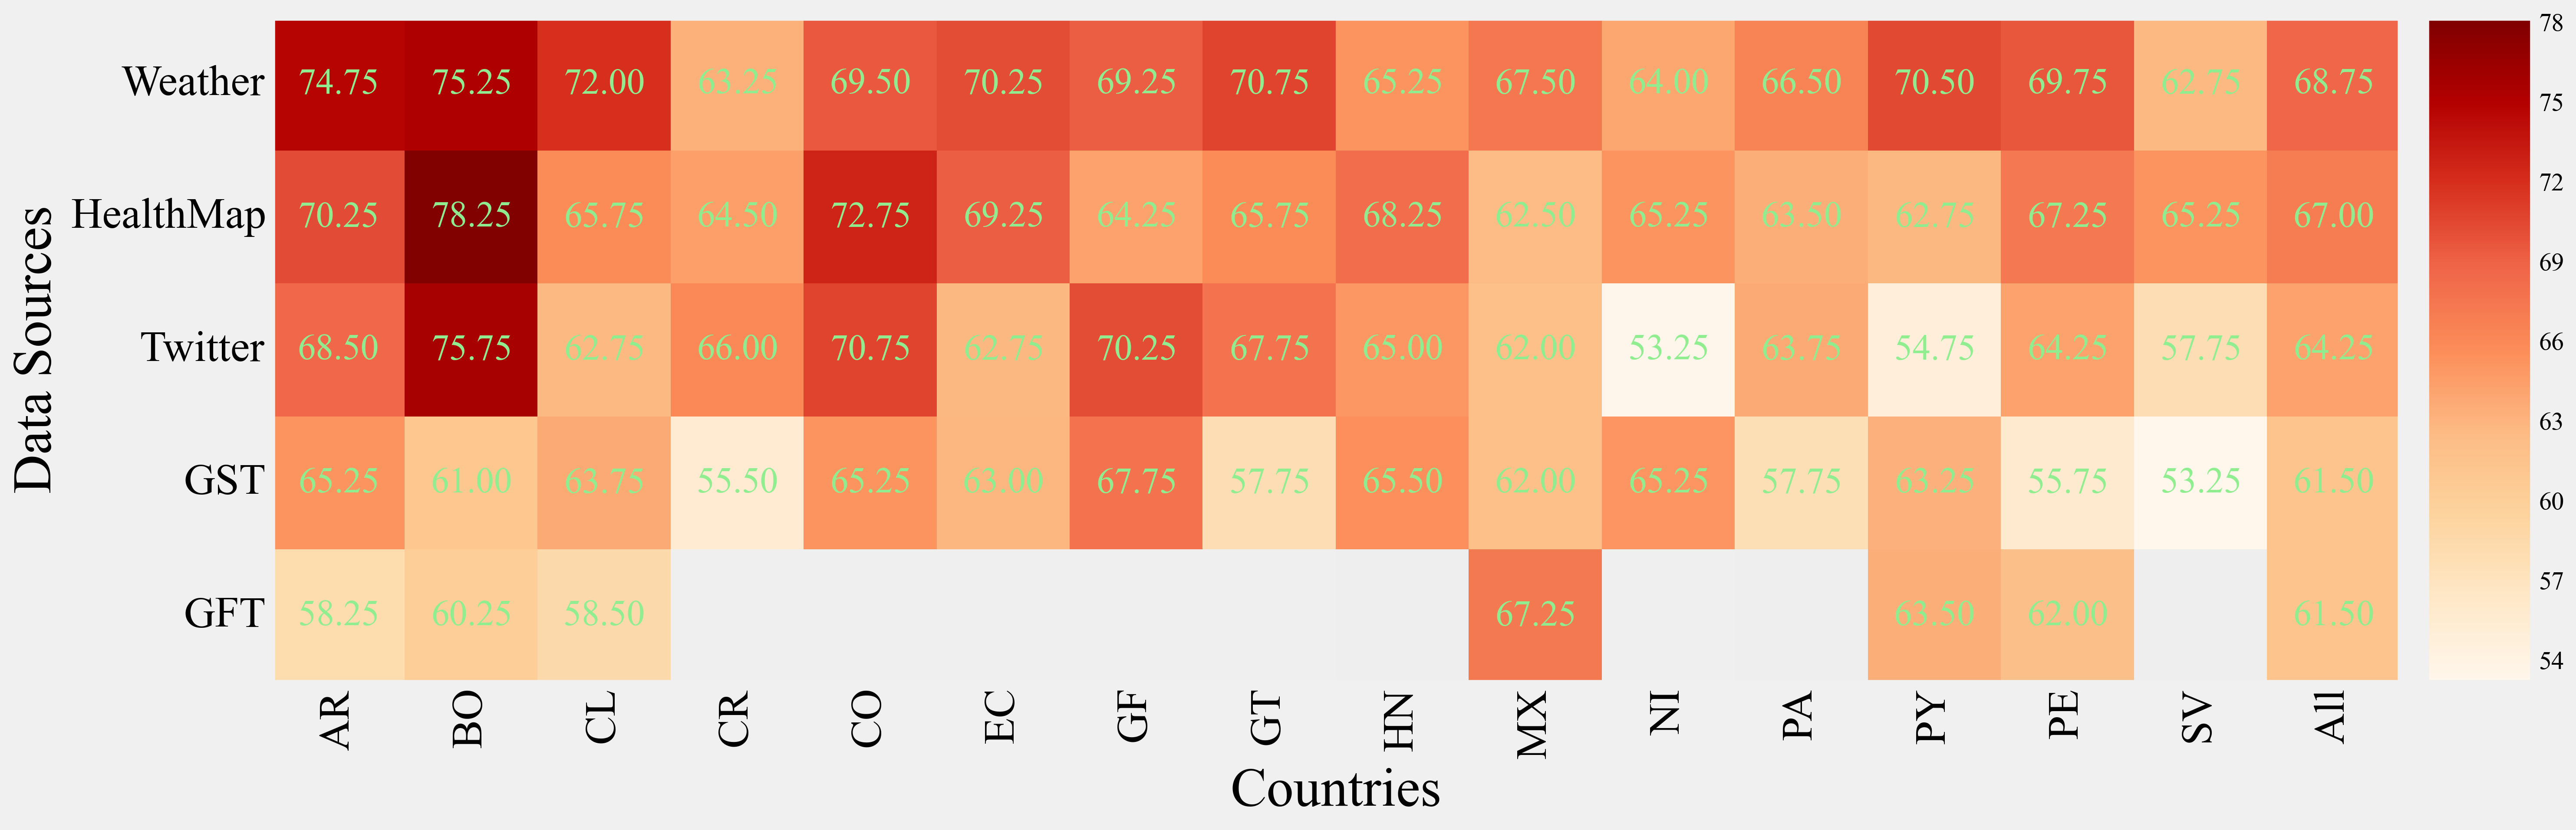
\includegraphics[height=0.12\textheight, width=0.55\textwidth]{./figs/singleSource.png}} 
  % \hspace{0.5em}
  % \subfloat[Multiple source prediction accuracy\label{2b}]{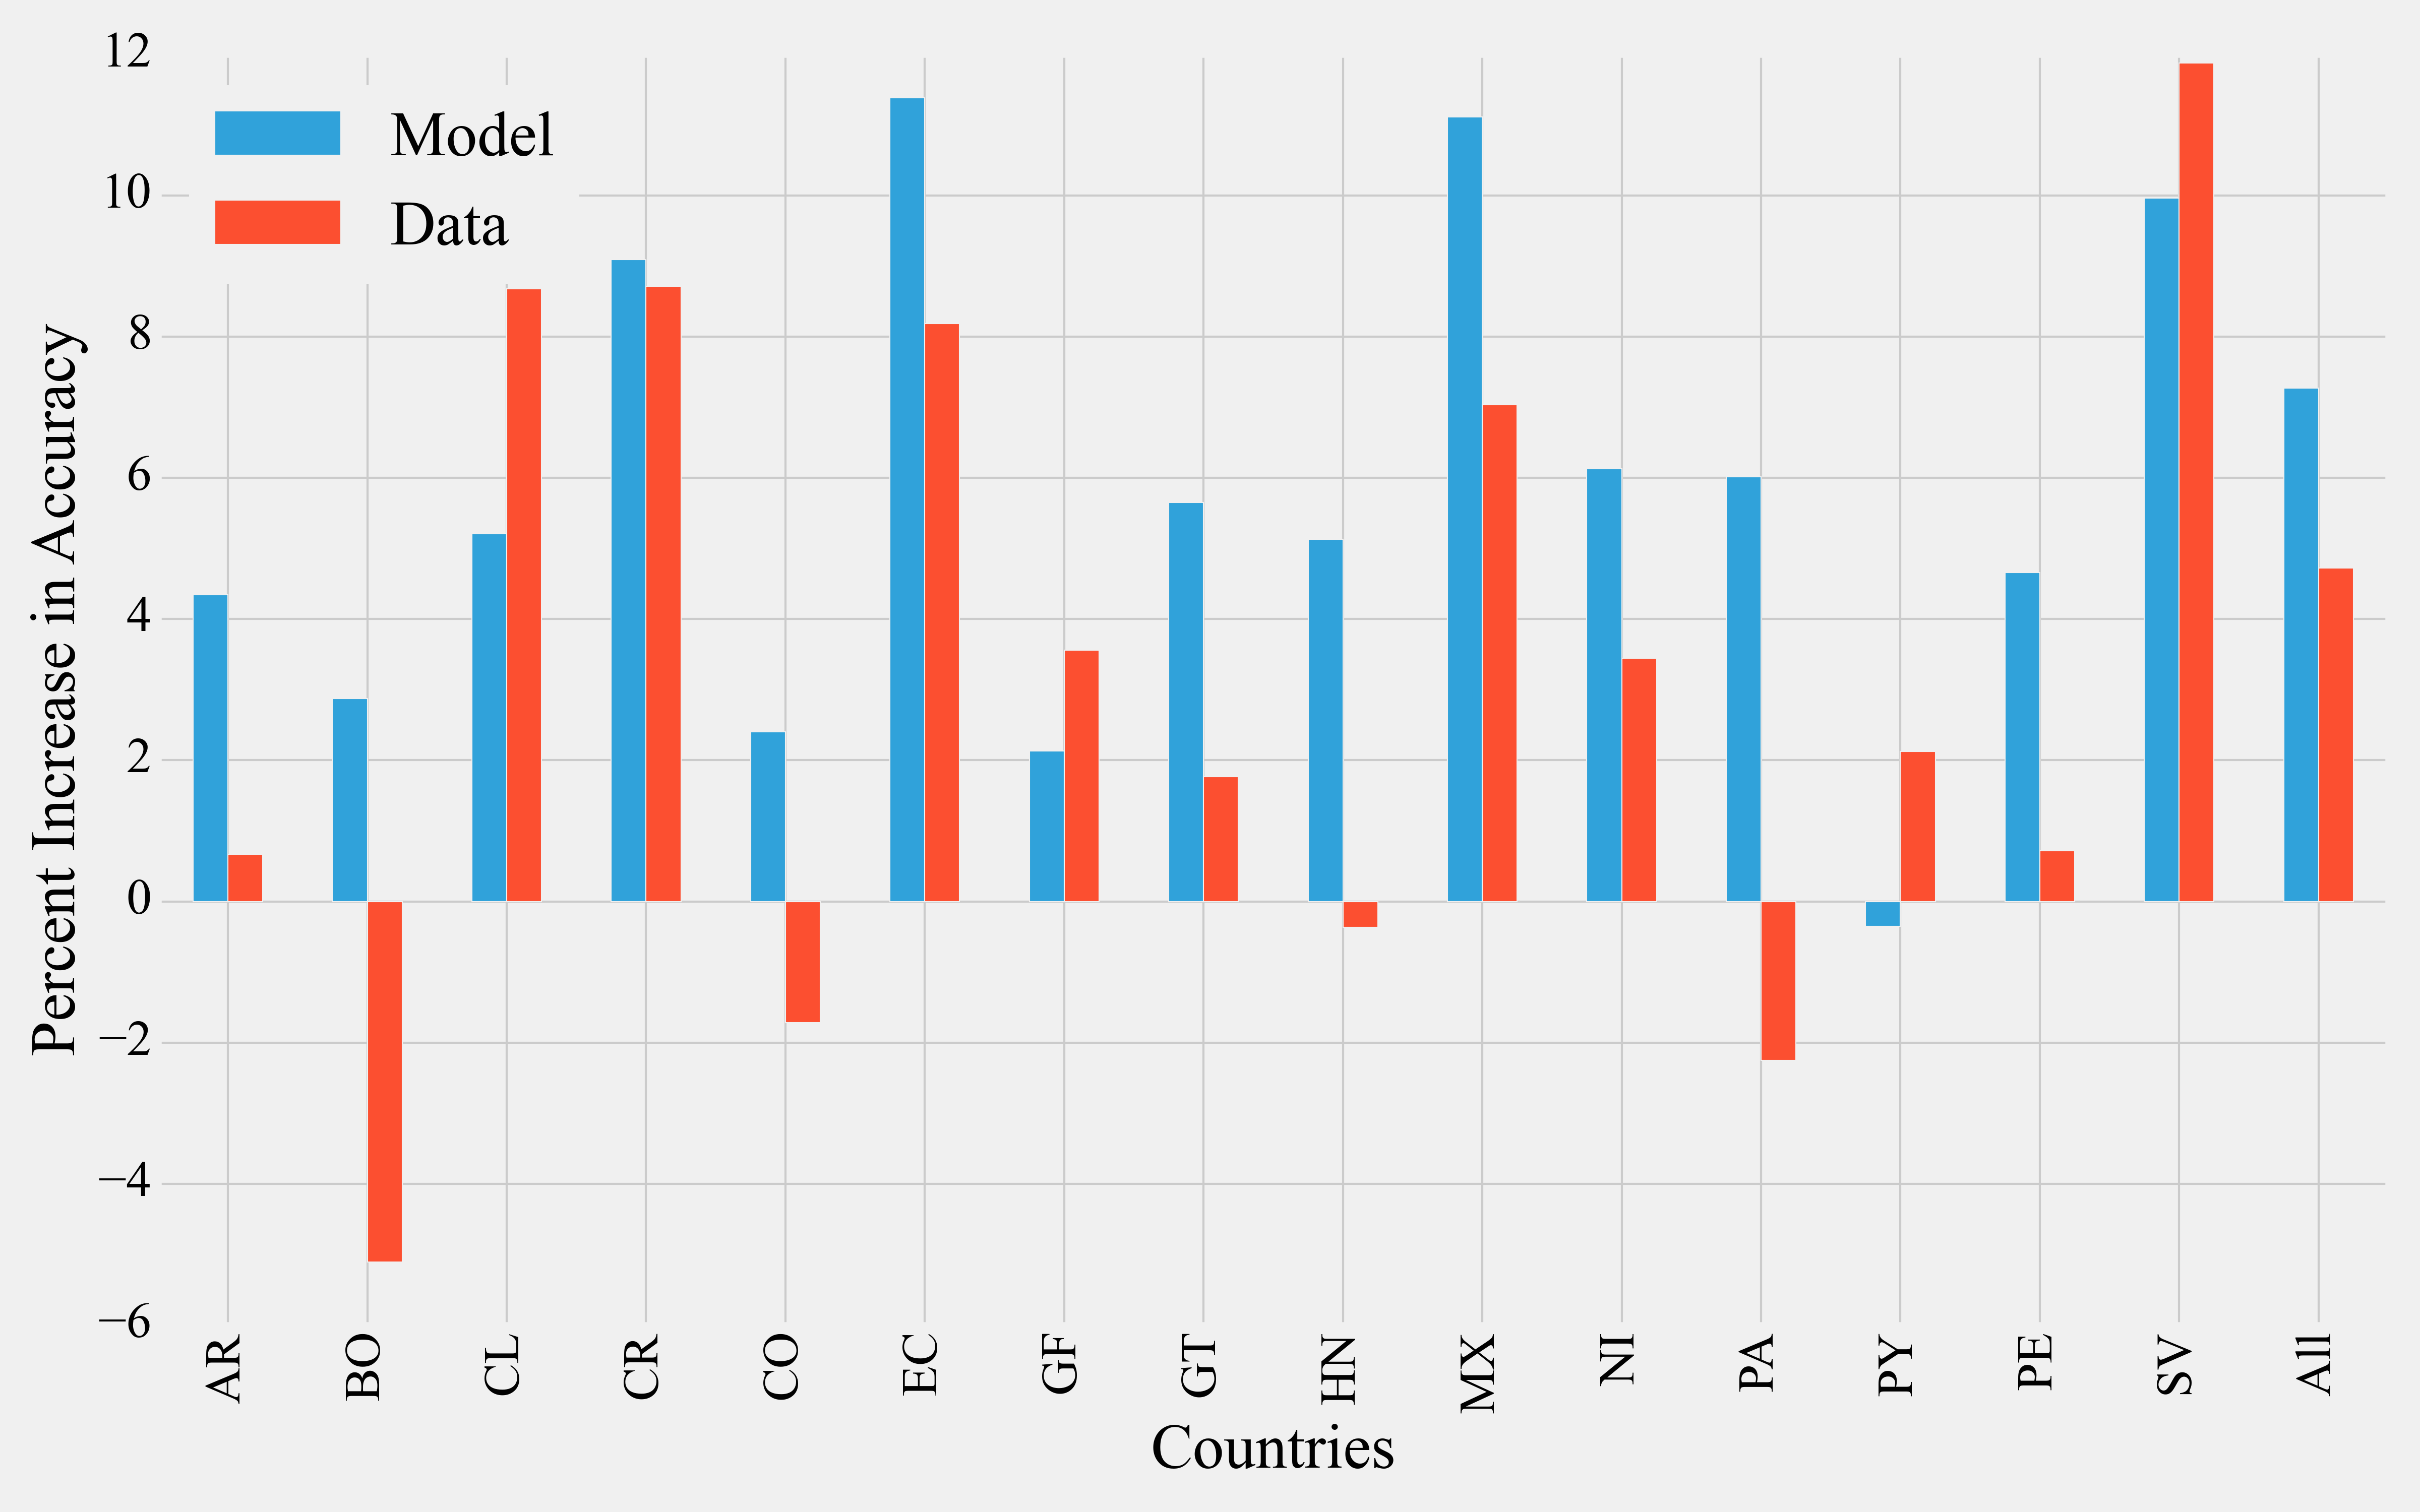
\includegraphics[height=0.12\textheight, width=0.35\textwidth]{./figs/ModelVsData.png}} 
  % \\
  % \subfloat[Percentage Accuracy reduction due to source ablation\label{2c}]{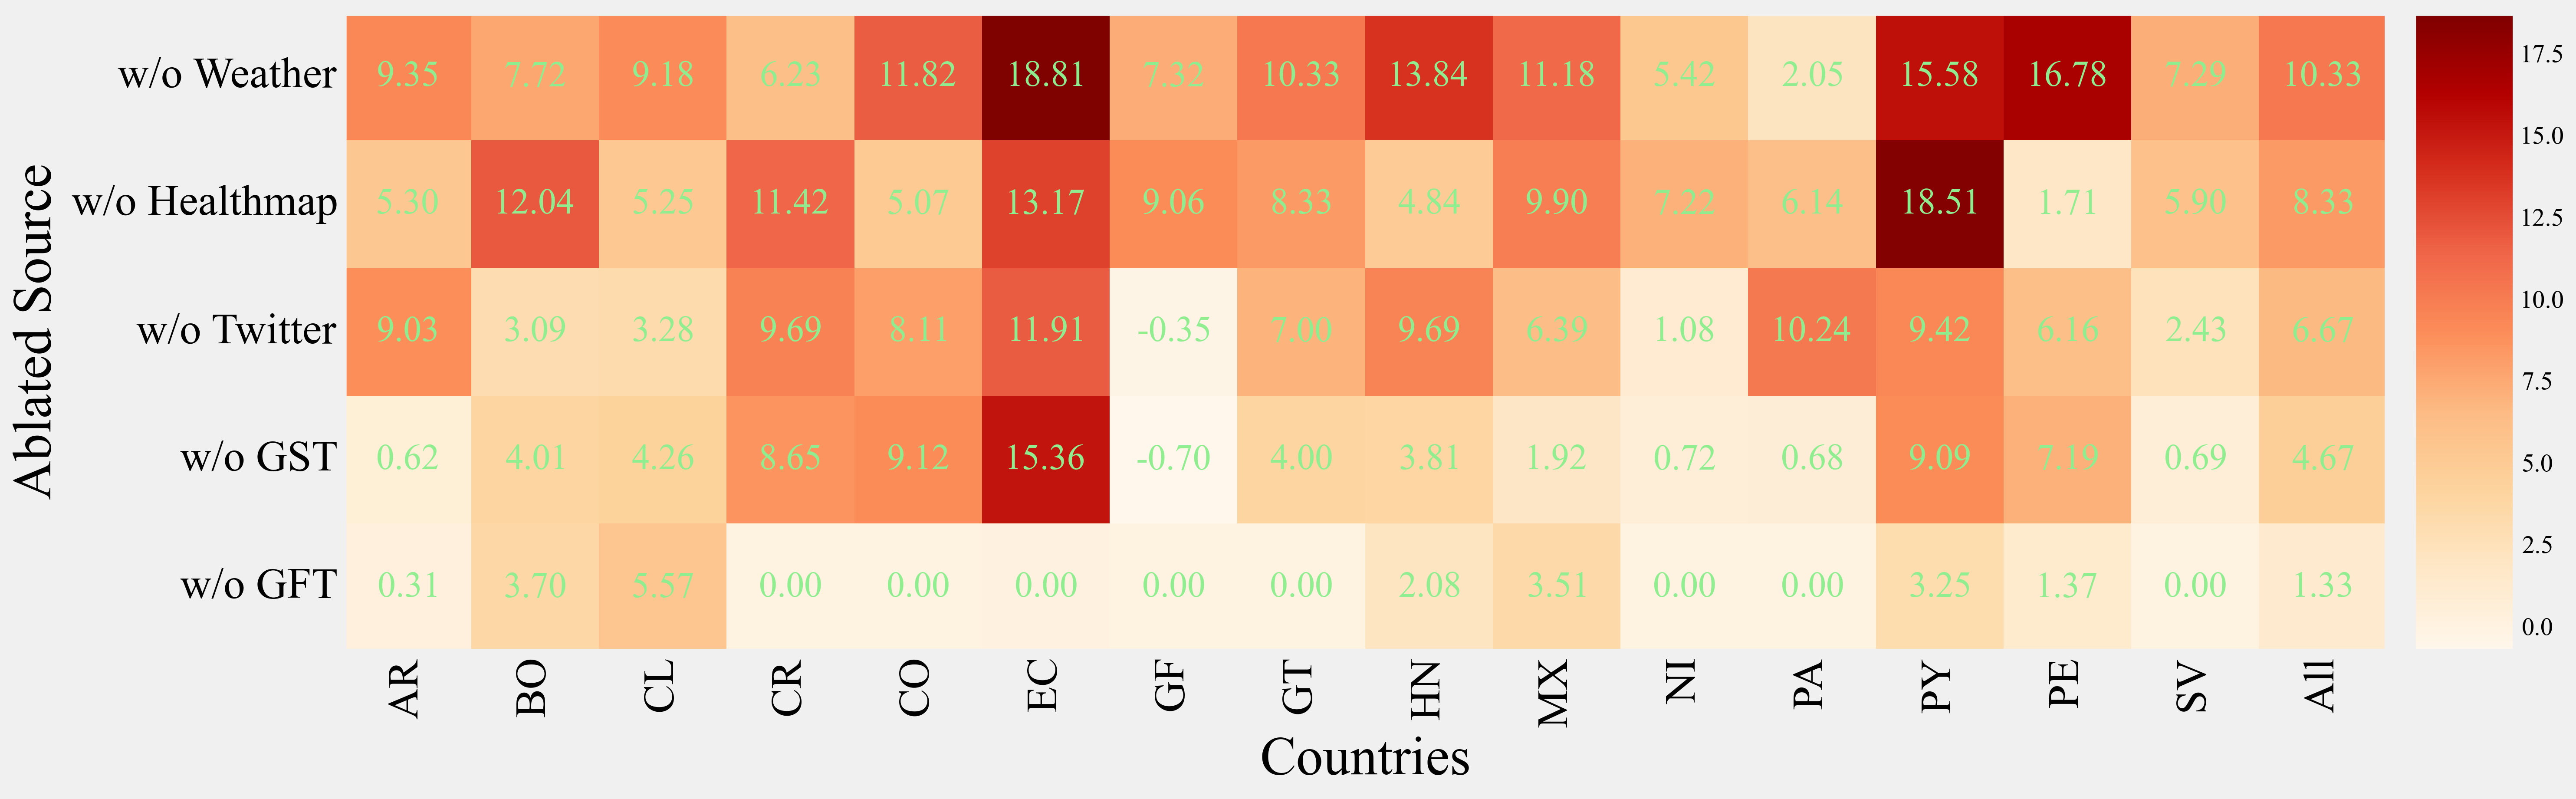
\includegraphics[height=0.10\textheight, width=0.45\textwidth]{./figs/Ablation.png}}
  % \hspace{0.5em}
  % \subfloat[Segregation: Prediction accuracy\label{2d}]{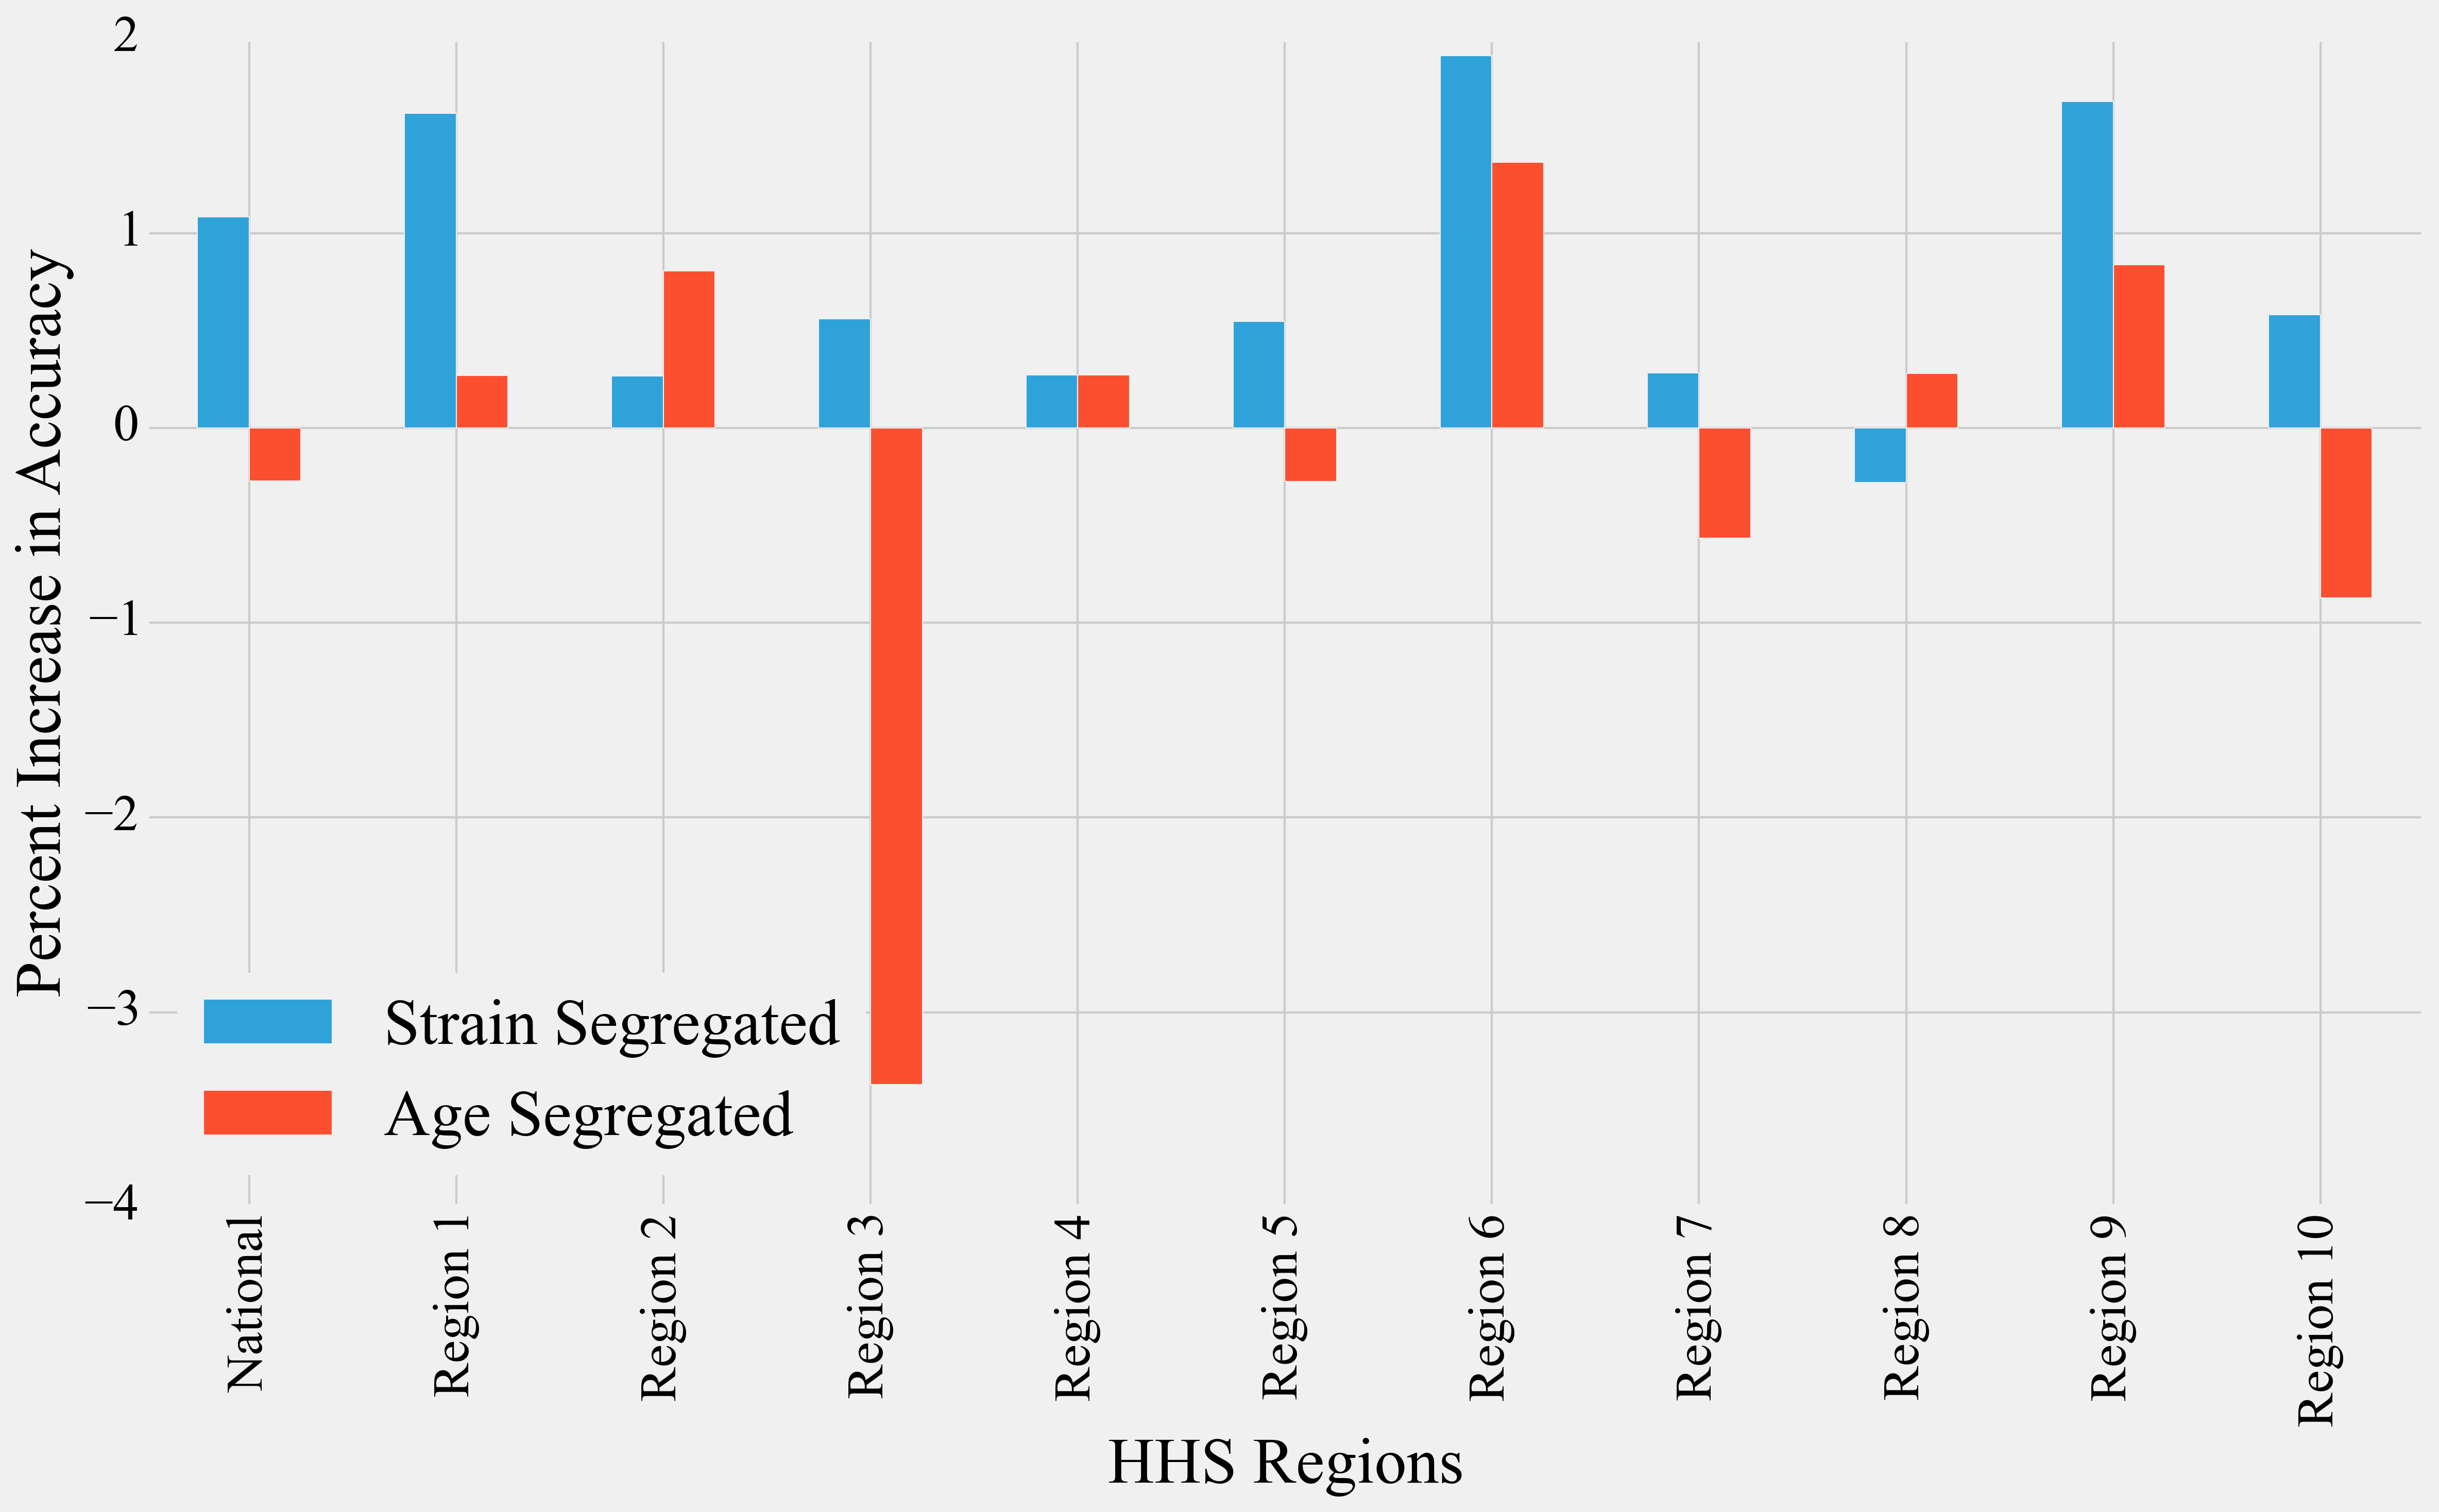
\includegraphics[height=0.10\textheight, width=0.25\textwidth]{./figs/FluSegregation.png}} 
  % \hspace{0.5em}
  % \subfloat[Instability Correction\label{2e}]{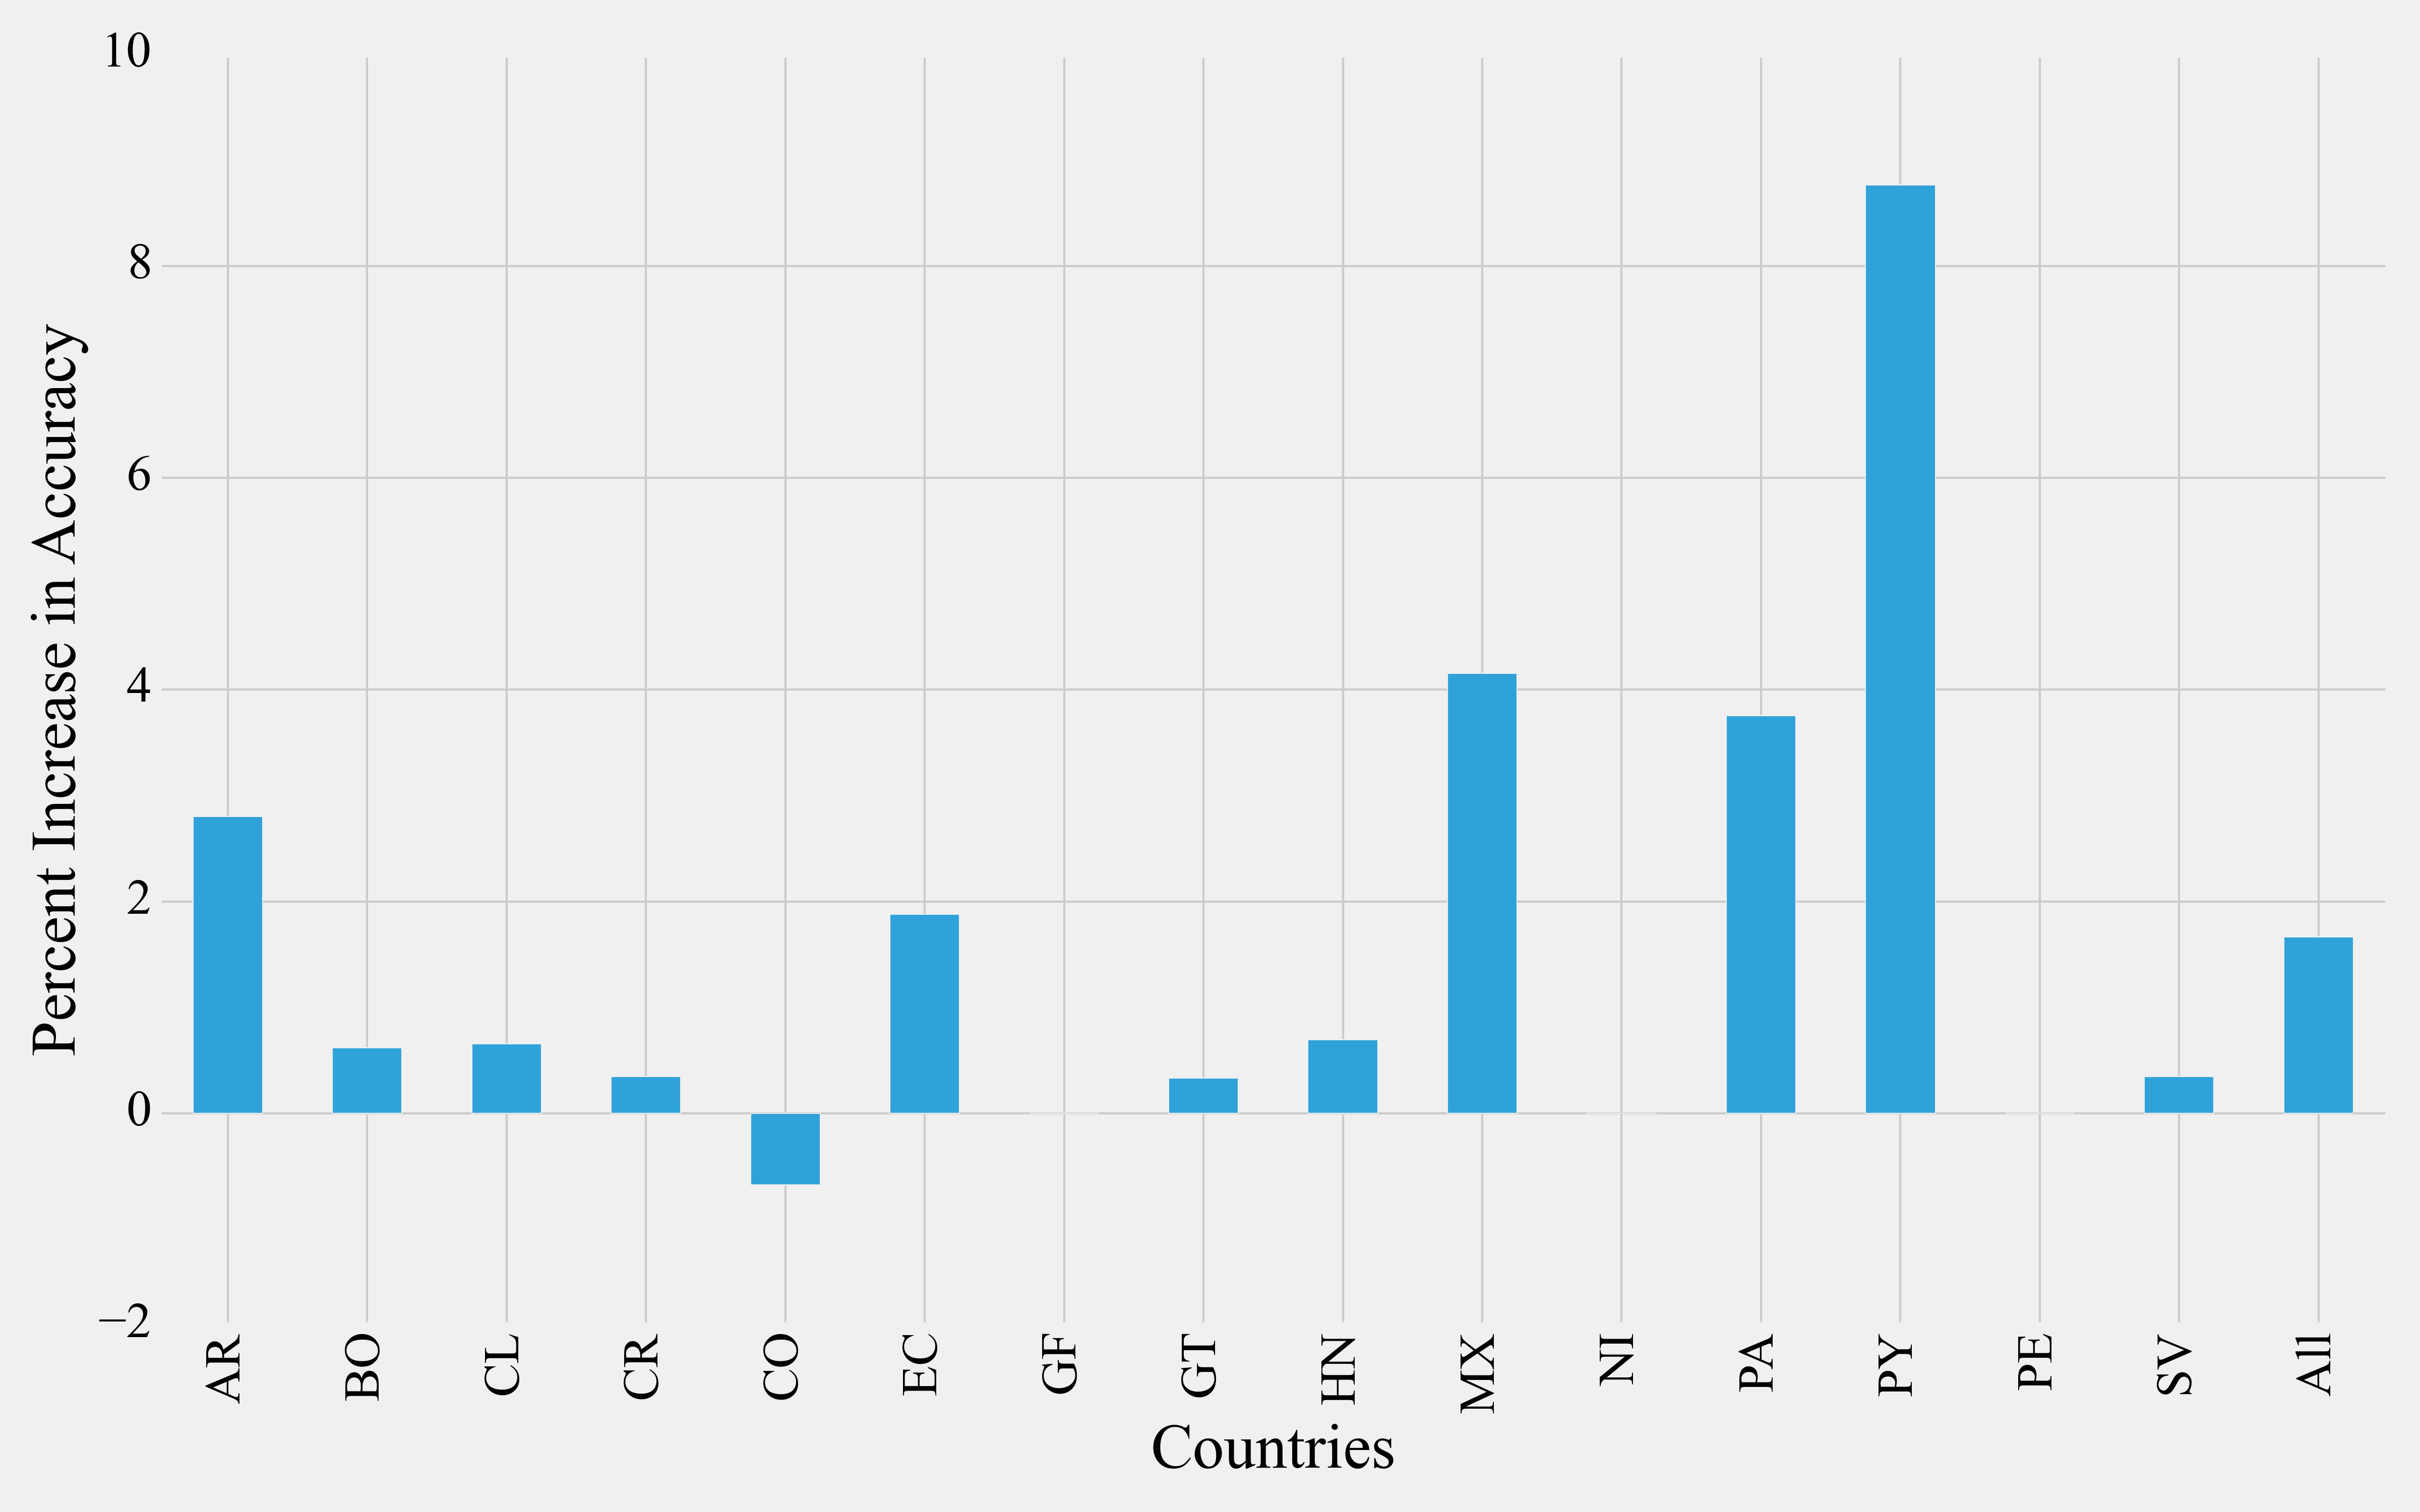
\includegraphics[height=0.10\textheight, width=0.25\textwidth]{./figs/PahoCorrection.png}} \\
  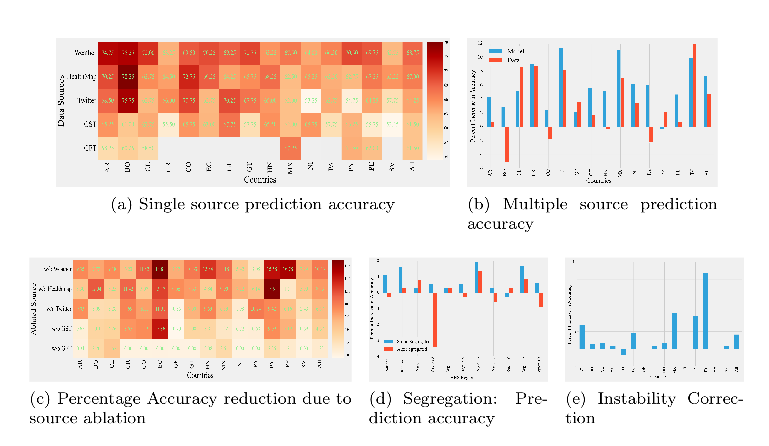
\includegraphics[width=0.96\linewidth]{./figs/perf_figs.eps}

  \caption{\textbf{Forecast accuracy under various conditions.}
  (a) \textit{Single Source:}
  Forecast accuracy for each individual source (Weather, Healthmap, 
  Twitter, Google Flu Trends and Google Search Trends). No particular 
  source is the best for all countries.
  (2) \textit{Multiple Sources:}
  Percent increase in forecast accuracies while combining multiple sources at 
  Model level and at Data level over best single source forecasts.
  Model level gives better overall performance.
  (c) \textit{Ablation test:}
  Percent reduction in forecast accuracies while 
  removing one source at a time from the Model fusion. 
  Removing a source can lead to better performance for some
  countries.
  (d) \textit{Segregation Test:}
  Percent increase in forecast accuracies for US ILI data considering 
  segregation by age and by subtype over unsegregated forecasts.
  Segregated methods show better accuracy.
  (e) \textit{Instability Correction:}
  Percent increase in forecast accuracies
  for different countries after correction over uncorrected forecasts.
  Significant improvement can be seen for countries like Argentina and 
  Paraguay.
  \label{fig2}
  }
\end{figure}

\section*{Surveillance Characteristics}
Flu surveillance networks exhibits several unique traits which can further be
modulated by regions/time period of interest. An effective flu forecasting 
system needs to pay careful attention to such characteristics. We discuss some
of the more important, but often overlooked, aspects of the surveillance
characteristics in the following sections.

\subsection*{Surveillance networks do not measure the same quantity}
Influenza-like Illnesses (ILI), tracked by many agencies such as CDC, PAHO, and
WHO~\cite{cdc,paho,who}, is a category designed to capture severe respiratory
disease, like influenza (flu), but also includes many other less severe
respiratory illness due to their similar presentation. Surveillance methods
often vary between agencies. Even for a single agency, there may be different
networks (such as outpatient based and lab sample based) tracking ILI/Flu.
While outpatient reporting networks such as ILINet aim to measure exact case
counts for the regions under consideration, lab surveillance networks such as
WHO NREVSS (used by PAHO) seek to confirm and identify the specific strain.  In
the absence of a clinic based surveillance system, lab-based systems can
provide estimates at per ``X'' population level; however making an estimate of
actual influenza flu cases from these systems is challenging~\cite{cdc}.
Furthermore, surveillance reports are often non-representative of actual ILI
incidence (see. ``epidemic data pyramid'') and can often suffer from variations
such as holiday periods where behavior of people visiting hospitals changes
from other weeks (see.  ``Christmas effect'' in supplementary material).
Additionally, the number of cases represented by a single positive lab sample
in a densely populated country with wide lab network coverage necessarily
differs from one in a more resource constrained lab surveillance system. For
example, in the US, the CDC reports percentage positive ILI for ILINet (an
outpatient reporting network) and for WHO NREVSS (based on lab samples). While
both networks are designed for different purposes and provide valuable
information for forecasting, they exhibit significant phase differences (see
Fig~\ref{fig1}a).  and, it is essential for forecasters to distinguish between
surveillance networks and their intricacies.  This difference is especially
important when conducting cross-correlation studies between different countries
(e.g., geographically nearby tropical countries may have similar underlying ILI
activity) or even between two different networks for the same country.

\subsection*{Flu is not ILI. ILI is plural. Geographical diversity must be
modeled}
Many surveillance systems for influenza report on Influenza like Illnesses
(ILI)~\cite{cdc} which is based on symptoms: fever (temperature of 100°F or
greater) and cough and/or sore throat.  This general classification is easier
to gather than more expensive and labor-intensive virological tests; however,
this definition means that multiple influenza strains and respiratory
infections are aggregated together. Such aggregation poses difficulties in
modeling because different strains of the flu exhibit different seasonal
characteristics (see Fig~\ref{fig1}b) where Flu A shows significantly different
phase than Flu B).  Consequently, a single forecasting model is unlikely to
capture the behavior of the overall epicurve. Our recommendation is to not
treat ILI as an atomic illness and instead predict for sub-strains if data at
required resolution(s) is available. Our experiments suggest that such
breakdown by strains can produce better quality predictions by accounting for
phase shifts between them (see Fig~\ref{fig2}d).

Similarly, building models at the national level without
considering differences in geography is likely to lead to erroneous results as
ILI characteristics are again shifted and scaled differently across regions. In
a geographically diverse country such as the United States, ILI seasonal curves
are consistently out of phase between different HHS regions as well as the
national curve. Further, a single region (e.g., HHS region 10 which subsumes
states such as Alaska and Washington) can be composed of non-contiguous land
masses which may make any assumption about uniformity in ILI profiles
inaccurate.

\subsection*{Surveillance data is not stable}
Epidemiologists who work with surveillance data know that, while useful, they
are often delayed and can be candidates for revision/updating for several weeks
after initial publication. The lag between initial publication and final
revision can be as small as 2 weeks (e.g., for CDC ILINet data) or can wildly
fluctuate (for example, PAHO reports for some Latin American countries such as
Argentina, Colombia and Mexico can take more than 10 weeks to settle. On the
other hand, PAHO reports stabilize within 5 weeks for countries such as Chile,
Costa Rica and Peru (see Fig~\ref{fig1}c).  The reason for such discrepancies
has to do with the maturity of the surveillance apparatus and the level of
coordination underlying public health reporting. Most works on forecasting do
not account for such instability. In essence, we are forecasting a moving
target and recent research~\cite{fischhoff2014communicating} suggests that
modeling such uncertainty directly in a forecasting model can significantly
improve performance. In particular, a stabilization or auto-correction term can
be inferred by conducting a regression for the final estimate as a function of
the intermediate values (and their times of publication)(see Fig~\ref{fig2}e).
One could devise more intricate algorithms that take into account cross-country
correlations and country-specific societal factors to correct for imperfections
in surveillance. 

\subsection*{Surveillance data collection practices are not uniform}
Even within a surveillance framework, there are systematic deviations in
coverage as well as differential lags in updates. Surveillance reporting has
been known to taper off or stop altogether during the post-peak part of the
season. For example, as is evident from Fig~\ref{fig1}d, the number of
providers who reported to US CDC ILINet surveillance tapers off towards the end
of the ILI season week (for US, calendar week 40 corresponds to first ILI
season week~\cite{cdc}).  Specifically, the inflection point of the average
curve occurs at week 33. Such effects can possibly be attributed to resource
re-allocation due to reduced interest in post-peak activities. This
necessitates modelers to make a distinction between expected ILI/flu curves and
the observed data for different parts of the season. Some efforts have been
made to account for such systematic deviations by either correcting their
estimates to match the surveillance reports~\cite{chakraborty2014forecasting}
or by explicitly modeling surveillance errors~\cite{shaman2013real}.  More
explicit data about the detailed structure of the surveillance system would
benefit these corrections.

\section*{Forecasting Practices}

\subsection*{There is no community agreement on measure(s) of performance
– forecasting reason}
Measuring forecasting skill is dependent on the actual use of the forecasts,
which varies widely. Not surprisingly, there is no accepted measure of
forecasting performance. We conducted a survey~\cite{matsubara2014funnel} where
we identified 7 different metrics for around 10 different quantities each
evaluating a different facet of flu. Moreover, evaluations often involve
multiple criteria, can include subjective components, and present trade-offs
where the balance of preferences is not well articulated. A vanilla
mean-squared error criterion will lead to a model with a tendency to
under-predict the peaks when trained uniformly over complete seasons. However,
if agencies are more interested in peak characteristics such a measure can be
modified to penalize deviations around peak more severely. Thus understanding
the requirements of health agencies is essential to generate meaningful
forecasts. Additionally, quantifying forecasting uncertainty and presenting the
same~\cite{tabataba2015smq} in a meaningful manner is of prime importance to
facilitate actionable strategies from health agencies.

\subsection*{The best case count predictor might not capture seasonal characteristics}
Forecasting tournaments provide much needed impetus to improving the
state-of-the-art of the field but viewing ILI prediction as machine learning or
regression problem misses the big picture. In particular, the best algorithm
according to a sum-of-squared-error or classical goodness-of-fit measure might
completely miss the most important seasonal characteristics such as the start
epiweek of the season, peak epiweek, and peak value - indicators likely to be
more important for public health and infection control purposes. 

\subsection*{Most published literature focuses on retrospective evaluations of forecasting methods}
To the best of our knowledge, the CDC and IARPA OSI competitions are the only
two competitions that truly involve forecasting into the future. Participants
were required to submit time-stamped forecasts that must arrive before the
event date (and thus certainly before the surveillance data becomes available).
In contrast, almost all published literature focuses on retrospective analysis
on flu seasons past~\cite{hall2007}.
The benefit of hindsight affords the ability to tune
models indefinitely, and out-of-sample testing is no substitute for
forecasting. Dangers include not just overfitting but also vulnerability to
model drift over time.

\subsection*{Many forecasting projects are not predicting into the future; they are really nowcasting, or near-casting}
Due to the delays and updates inherent in surveillance data, a ``forecasting''
project predicting one or two weeks into the future is in essence a
``nowcasting''~\cite{lampos2012nowcasting} system.  Understanding this aspect
is crucial as it could lead to intelligent strategies of handling surrogate
information~\cite{Preis140095} such as weather data and social network sensors.
Since surrogate sources are typically real-time, when performing nowcasting one
can ideally complement knowledge of last known surveillance data with the
current surrogates and hence find a direct estimate of the surveillance data.
On the other hand a prediction engine interested in forecasting the peak of the
flu season (say 7 weeks in advance), does not have the same liberty. Some
researchers have used data assimilation
techniques~\cite{lampos2012nowcasting,ronni2015empbayes} to incorporate
knowledge about weather data to provide ILI forecasts. Intelligent assimilation
techniques can be developed to incorporate weather forecasts (which are also
available) and reduce the error bounds while predicting for more than, say,
four weeks in advance. 

\subsection*{Bigger Data is not always Better Data}
There is now a wealth of syndromic surveillance and physical indicators
available for forecasting the flu such as weather, news reports, web search
query volumes (GFT, GST), Twitter chatter~\cite{chakraborty2014forecasting} and
Wikipedia logs~\cite{mciver2014wikipedia,hickman2015wikipedia}.  Pitfalls in
big data analysis without understanding the underlying system biases have been
well-documented (e.g., for GFT, see~\cite{lazer2014parable}).  We evaluated
diverse data sources for flu forecasting in 15 Latin American countries
(Fig~\ref{fig2}a) and have considered both data-level fusion and model-level
fusion. The former concatenates all data sources and renders them in a common
denominator format before modeling. Model-level fusion builds separate models
with each source and combines their forecasts leveraging selective
superiorities. As Fig~\ref{fig2}b shows, model-level fusion performs better
than data-level fusion. “Ablation tests” (see Fig~\ref{fig2}c) show that
physical indicators are consistently the more important predictor than social
indicators. Inclusion of some data sources can actually lead to reduced
performance for specific countries (e.g., Google Search Trends for French
Guiana).

\section*{Conclusion}
Infectious disease forecasting is a rapidly emerging field. The challenges
reported here pertain to how data from surveillance systems can be modeled as
well as how forecasting standards need to mature. While we have focused on flu
forecasting here, these challenges translate to other diseases as well. We
advocate increased efforts in fostering a community of forecasters and
converging on a common understanding of shared concerns and approaches forward.
We also argue for easier availability of surveillance data and surrogate
sources in raw forms, at all possible spatial and temporal granularities.
Skilled forecasting research can significantly aid in the translation of
research results into the hands of public policy professionals and decision
makers.

\section*{Supporting Information}

\paragraph*{S1 Appendix.}
\label{S1_Appendix}
Datasets and associated code snippets for this article is archived at the
publicly accessible github page \url{http://prithwi.github.io/how_not2_flu}.


\section*{Acknowledgments}
This work is supported by the Intelligence Advanced Research Projects Activity
(IARPA) via Department of Interior National Business Center (DoI/NBC) contract
number D12PC000337and by the Defense Threat Reduction agency (DTRA) via the
CNIMS Contract HDTRA1-11-D-0016-000. The US Government is authorized to
reproduce and distribute reprints of this work for Governmental purposes
notwithstanding any copyright annotation thereon. Disclaimer: The views and
conclusions contained herein are those of the authors and should not be
interpreted as necessarily representing the official policies or endorsements,
either expressed or implied, of IARPA, DoI/NBC, DTRA, or the US Government.

\nolinenumbers

% \bibliographystyle{plos2015}
\bibliography{references}
\end{document}
